\documentclass[11pt,a4paper,oneside]{report}             % Single-side
%\documentclass[11pt,a4paper,twoside,openright]{report}  % Duplex

%\PassOptionsToPackage{chapternumber=Huordinal}{magyar.ldf}
\usepackage{t1enc}
\usepackage[utf8]{inputenc}
\usepackage{amsmath}
\usepackage{amssymb}
\usepackage{enumerate}
\usepackage[thmmarks]{ntheorem}
\usepackage{graphics}
\usepackage{epsfig}
\usepackage{listings}
\usepackage{color}
%\usepackage{fancyhdr}
\usepackage{lastpage}
\usepackage{anysize}
\usepackage[magyar]{babel}
\usepackage{sectsty}
\usepackage{setspace}  % Ettol a tablazatok, abrak, labjegyzetek maradnak 1-es sorkozzel!
\usepackage[hang]{caption}
\usepackage{hyperref}

%--------------------------------------------------------------------------------------
% Main variables
%--------------------------------------------------------------------------------------
\newcommand{\vikszerzo}{Kovács Ádám}
\newcommand{\vikszerzos}{Gémes Andrea Kinga}
\newcommand{\vikkonzulens}{Dr.~Recski Gábor}
\newcommand{\vikcim}{Semantic parsing with graph transformations}
\newcommand{\viktanszek}{Department of Automation and Applied Informatics}
\newcommand{\vikdoktipus}{Scientific Student’s Assosiactions Report}
\newcommand{\vikdepartmentr}{Kovács Ádám}

%--------------------------------------------------------------------------------------
% Page layout setup
%--------------------------------------------------------------------------------------
% we need to redefine the pagestyle plain
% another possibility is to use the body of this command without \fancypagestyle
% and use \pagestyle{fancy} but in that case the special pages
% (like the ToC, the References, and the Chapter pages)remain in plane style

\pagestyle{plain}
%\setlength{\parindent}{0pt} % ?ttekinthet?bb, angol nyelv? dokumentumokban jellemz?
%\setlength{\parskip}{8pt plus 3pt minus 3pt} % ?ttekinthet?bb, angol nyelv? dokumentumokban jellemz?
\setlength{\parindent}{12pt} % magyar nyelv? dokumentumokban jellemz?
\setlength{\parskip}{0pt}    % magyar nyelv? dokumentumokban jellemz?

\marginsize{35mm}{25mm}{15mm}{15mm} % anysize package
\setcounter{secnumdepth}{0}
\sectionfont{\large\upshape\bfseries}
\setcounter{secnumdepth}{2}
\singlespacing
\frenchspacing

%--------------------------------------------------------------------------------------
%	Setup hyperref package
%--------------------------------------------------------------------------------------
\hypersetup{
    bookmarks=true,            % show bookmarks bar?
    unicode=false,             % non-Latin characters in Acrobat?s bookmarks
    pdftitle={\vikcim},        % title
    pdfauthor={\vikszerzo},    % author
    pdfsubject={\vikdoktipus}, % subject of the document
    pdfcreator={\vikszerzo},   % creator of the document
    pdfproducer={Producer},    % producer of the document
    pdfkeywords={keywords},    % list of keywords
    pdfnewwindow=true,         % links in new window
    colorlinks=true,           % false: boxed links; true: colored links
    linkcolor=black,           % color of internal links
    citecolor=black,           % color of links to bibliography
    filecolor=black,           % color of file links
    urlcolor=black             % color of external links
}

%--------------------------------------------------------------------------------------
% Set up listings
%--------------------------------------------------------------------------------------
\lstset{
	basicstyle=\scriptsize\ttfamily, % print whole listing small
	keywordstyle=\color{black}\bfseries\underbar, % underlined bold black keywords
	identifierstyle=, 					% nothing happens
	commentstyle=\color{white}, % white comments
	stringstyle=\scriptsize\sffamily, 			% typewriter type for strings
	showstringspaces=false,     % no special string spaces
	aboveskip=3pt,
	belowskip=3pt,
	columns=fixed,
	backgroundcolor=\color{lightgray},
} 		
\def\lstlistingname{lista}	

%--------------------------------------------------------------------------------------
%	Some new commands and declarations
%--------------------------------------------------------------------------------------
\newcommand{\code}[1]{{\upshape\ttfamily\scriptsize\indent #1}}

% define references
\newcommand{\figref}[1]{\ref{fig:#1}.}
\renewcommand{\eqref}[1]{(\ref{eq:#1})}
\newcommand{\listref}[1]{\ref{listing:#1}.}
\newcommand{\sectref}[1]{\ref{sect:#1}}
\newcommand{\tabref}[1]{\ref{tab:#1}.}

\DeclareMathOperator*{\argmax}{arg\,max}
%\DeclareMathOperator*[1]{\floor}{arg\,max}
\DeclareMathOperator{\sign}{sgn}
\DeclareMathOperator{\rot}{rot}
\definecolor{lightgray}{rgb}{0.95,0.95,0.95}

\author{\vikszerzo}
\title{\viktitle}
\includeonly{
	titlepage,%
	declaration,%
	abstract,%
	introduction,%
	compsem,%
	4lang,%
	Yuanfudao-system, %
	chapter1,%
	chapter2,%
	chapter3,%
	acknowledgement,%
}
%--------------------------------------------------------------------------------------
%	Setup captions
%--------------------------------------------------------------------------------------
\captionsetup[figure]{
%labelsep=none,
%font={footnotesize,it},
%justification=justified,
width=.75\textwidth,
aboveskip=10pt}

\renewcommand{\captionlabelfont}{\small\bf}
\renewcommand{\captionfont}{\footnotesize\it}

%--------------------------------------------------------------------------------------
% Table of contents and the main text
%--------------------------------------------------------------------------------------
\begin{document}
\singlespacing

\pagenumbering{arabic}
\onehalfspacing
%--------------------------------------------------------------------------------------
%	The title page
%--------------------------------------------------------------------------------------
\begin{titlepage}
\begin{center}

\includegraphics[width=60mm,keepaspectratio]{figures/BMElogo.png}\\
\vspace{0.3cm}
\textbf{Budapesti Műszaki és Gazdaságtudományi Egyetem}\\
\textmd{Villamosmérnöki és Informatikai Kar}\\
\textmd{\viktanszek}\\[5cm]

\vspace{0.4cm}
{\huge \bfseries \vikcim}\\[0.8cm]
\vspace{0.5cm}
\textsc{\Large \vikdoktipus}\\[4cm]

\begin{tabular}{cc}
 \makebox[7cm]{\emph{Author}} & \makebox[7cm]{\emph{Supervisor}} \\
 \makebox[7cm]{\vikszerzo} & \makebox[7cm]{\vikkonzulens} \\
 \makebox[7cm]{\vikszerzos}
\end{tabular}

\vfill
{\large \today}
\end{center}
\end{titlepage}



%----------------------------------------------------------------------------
% Abstract in hungarian
%----------------------------------------------------------------------------
\chapter*{Kivonat}\addcontentsline{toc}{chapter}{Kivonat}
%--------------------------------------------------------------------------------------
% semantic parsing, graftranszformacio altalaban
A szemantikai elemzés célja, hogy természetes nyelvi adathoz
készíthessünk szemantikai reprezentációt, így tudjuk modellezni a szöveg jelentését. Ha a nyelvi
jelentést fogalmak irányított gráfjaival reprezentáljuk, ezeket pedig a mondat szintaktikai
szerkezetét reprezentáló fákból kell előállítanunk, akkor a teljes feladat egyetlen komplex gráftranszformációként
definiálható.

%--------------------------------------------------------------------------------------
% machine comprehension
A természetes nyelv szemantikájának reprezentációját ritkán használják közvetlenül a state-of-the art rendszerekben népszerű szemantikai feladatokra, mint a szemantikai hasonlóság mérése, vagy a gépi szövegértés. Ezek a rendszerek többnyire szó embeddingeket használnak a szavak jelentésének ábrázolására.
Ebben a dolgozatban mi gráf reprezentációkat és transzformációkat használunk, mint egyszerű ám hatékony eszközök az oksági viszony felismerésére, valamint leírunk egy módszert a \texttt{4lang} szemantikus elemzőrendszer (Recski:2016) használatára a 2018-as Semeval Task \textit{Machine comprehension using commonsense knowledge} kapcsán. Ez a feladat azt kívánja a résztvevőktől, hogy olyan rendszereket tanítsanak fel, amelyek ki tudják választani a megfelelő választ az egyszerű, több válaszlehetőséget kínáló kérdéseknél rövid eseményleíró szövegek elolvasása után. A tanító és teszt adat az \texttt{MCScript} adathalmaz (Ostermann et al., 2018) részhalmazából lett kinyerve.
A két legjobb rendszer, \texttt{HFL-RC} (Chen et al., 2018) és \texttt{Yuanfudao} egyenként $84,15\%$ és $83,95\%$ pontosságot ért el a teszt adaton.

%--------------------------------------------------------------------------------------
% baseline
Először bemutatunk egy hatékony baselinet ezen a feladaton csupán a szemantikus gráfok és a köztük lévő hasonlóságok felhasználásával. Ezt követően leírjuk a \texttt{Yuanfudao} (Wang et al., 2018) state-of-the art rendszert és az ezzel végzett kísérletezéseinket, amelyek során
%--------------------------------------------------------------------------------------
% rendszer, amivel foglalkoztunk
a baselineunkat extra featureként felhasználva javítottunk a neurális hálón. A rendszer kiválasztása magától értetődő volt, mivel a forráskód nyilvánosan elérhető és már sikeresen alkalmazott tudás alapú reprezentációt a szópárok közötti szemantikai kapcsolatokra, a \textit{ConceptNet}et.
Eredményeink azt mutatják, hogy ezzel a módosítással $0,5\%$ százalékpont növekedés érhető el és a \textit{ConceptNet} helyettesíthető a mi szemantikus modellünkkel.
\vfill

%----------------------------------------------------------------------------
% Abstract in english
%----------------------------------------------------------------------------
\chapter*{Abstract}\addcontentsline{toc}{chapter}{Abstract}
%--------------------------------------------------------------------------------------
% semantic parsing, graftranszformacio altalaban
The main task of semantic parsing is to automatically build semantic representation from the input, so we can model the meaning
of raw texts. If we model meaning as directed graphs of concept and we can build them from syntax trees that represent the structure of 
sentences, then we can define the whole process as one complex graph transformation.

%--------------------------------------------------------------------------------------
% machine comprehension
Representations of natural language semantics are rarely used explicitly in state-of-the art systems for popular semantics tasks such as measuring semantic similarity or machine comprehension. These systems mostly use word embeddings as representation of word meaning.

In this paper we use graphical representations and transformations as simple but powerful tools for recognizing entailment and we describe a method using semantic parsing system \texttt{4lang} (Recski:2016) and applying it on the 2018 Semeval Task \textit{Machine comprehension using commonsense knowledge}. This task requires participants to train systems that can choose the correct answer to simple multiple choice questions based on short passages describing simple chains of events. Data for both training and testing is extracted from the \texttt{MCScript} dataset (Ostermann et al., 2018). The top two systems, \texttt{HFL-RC} (Chen et al., 2018) and \texttt{Yuanfudao} achieved accuracy scores of $84.15\%$ and $83.95\%$ on the test data, respectively.

%--------------------------------------------------------------------------------------
% baseline
First we will present a strong baseline on this task using only semantic graphs and similarities among them, followed by 
a description of a state-of-the art system \texttt{Yuanfudao} (Wang et al., 2018) and our experiments with it where
%--------------------------------------------------------------------------------------
% rendszer, amivel foglalkoztunk
we used our baseline as an extra feature for improving the neural network. The choice of the system was obvious, because the source code is publicly available and it already employs successfully a knowledge base representing semantic relationships among pairs of words, \textit{ConceptNet}.
Our results suggest that these features achieve a .5 percentage point improvement, and the \textit{ConceptNet} could be replaced by our semantic model.
\vfill


\tableofcontents\vfill
\chapter{Introduction}
\label{chap:Introdu}
%----------------------------------------------------------------------------
\section{Natural Language Processing}
While computers can be easily programmed to understand structured data, such as tables and spreadsheets, it can be rather challenging for them
to understand human communication. Because there is a vast difference in the magnitude of the unstructured data compared to the structured ones, there is a high demand
for tools, that can deal with raw text. Thats where NLP comes in. It contains high variety of tools, that we have to use, when we need to deal with natural input.

Every day, we come into contact with human communication, we say a lot of words to other people, and they try to interpret them even when the context of the saying 
isn't necesseraily complete. The listeners can use their common knowledge to fill the needed information. We resolve ambiguities, misunderstanding, and can even understand words 
we have never heard before just from the context of the communication.
Even though these tasks are trivial for us, for a computer it can be really hard.

%--------------------------------------------------------------------------------------
% egyszer� multtol jelenig bevezeto
The interest in NLP research began in the 1950s, the early phase was mainly focused on MT (Machine Translation), because after the World War II, people
recognised the importance of the translation from one language to another, and hoped to do it automatically.
However MT is still a very difficult nowadays, so these researches discovered early the main challenges of the syntactic and semantic parsing.
As time passed, researches embraced new areas of NLP as more advanced technology and knowledge became available. Now that we live in a world where
computers and smartphones, collecting data became incredibly easy, as a result, statistical NLP drew attention because these models thrive off big data, but one cannot ignore 
simple rule based methods, which can also be a very powerful method, especially using them as a hybrid model with statistical methods.
%--------------------------------------------------------------------------------------
% r�vid nlp pipeline

Building NLP applications requires many levels of analysis.
The typical pipeline structured as follows:
\begin{itemize}
	\item First we need to tokenize our input text, which means breaking up the text into meaningful elements, especially into words
	\item After we tokenized our text, we need word analysis called \texttt{morphology}, which is concerned with the structure of words.
	\item Part of speech explains how a word is used in a sentence, and tagging is a process marking words to its particular part of speech.
	\item The main task of syntactic parsing is to analyze the grammatical structure of a sentence. Given a set of words, a parser forms units (subjects, verbs, etc..) according to some grammatical formalism.
	There are two main type of syntactic parsers:
	\begin{itemize}
		\item Consituency parsers produce trees, that represents the grammatical structure.
		\item Dependency parsers are the more popular nowadays. They represent the structure of a sentence as a dependency tree.
	\end{itemize}
	\item At this point we have various ways to analyze a text, but without modeling its \texttt{meaning}. Semantic is the study of meaning, and semantic parsing is a task to find a representation and assign it to the text. This task will be the main topic of my work.
\end{itemize}
%----------------------------------------------------------------------------
\chapter*{Computational Semantics}\addcontentsline{toc}{chapter}{Computational Semantics}
\label{sec:compsem}
%----------------------------------------------------------------------------
We use the word semantics in our ordinary language, when we want to discuss the meaning or an interpretation of a group of words within the boundaries of a certain context.
So we say that the semantics is the study of meaning, and if we talk about NLP it usually refers to the meaning of linguistic utterances.
The semantics of an utterance is closely connected to many scientific fields, such as philosophy, logic or knowledge representation.
Applications covered in this course so far are all possible without any explicit representation of what certain linguistic structures mean.
Even complex processes like syntactic parsing, or even machine translation can be ignorant of what each word, phrase or sentence means, i.e. what information it conveys to speakers of the language.
Other tasks rely heavily on semantics, they are the biggest tasks, where semantic technologies need to be used.

There are a few main applications that needs to be mentioned when we are talking of computational semantics:
\begin{itemize}
	\item \textbf{Question answering} is the process of generating meaningful answers to the user's question, using some kind of knowledge.
	\item \textbf{Recognizing entailment} is whether a statement implies another or not, it is closely connected to \textbf{machine comprehension}, which is the main focus of our work.
	\item \textbf{Personal assistants} such as Apple Siri or Alexa, they are heavily widespread nowadays, and every one of us has one with their phone.
	\item \textbf{Chatbots} are systems, that could somewhat carry a human-like conversation.
\end{itemize}
\section{Main tasks}
\subsection{Relation extraction}
In our modern world, the amount of information in need of processing is increasing every day, so the demand of automate the process of analyzing came through. The problem of building structured information from raw text is the task of Information Extraction (IE) \cite{Jurafsky:2009}.

After we gained structured information, it can be used by many other NLP task. Generally when we start an IE task, the first problem we have to deal is the classification of proper names, usually referred as Named Entity Recognition (NER) \cite{RelationE}. The next step is usually the coreference resolution, which is determining the relations between the Named Entities \cite{Jurafsky:2009}. This is where relation extraction comes in. It is the analysis that turns unstructured information into structured data. We need to identify the links between the entities. Finally we need the information for template filling, that involves filling the slots in some templates. Template filling can be used for many purposes:

\begin{itemize}
	\item professional profiles based on some Facebook pages, CVs
	\item product specifications
	\item identifying terrorist attacks
\end{itemize}

So as we discussed, RE aims to gather relations between NEs. Cullota \cite{Cullota06} define relation extraction as:
\begin{quotation}
	“the task of discovering semantic connections between entities. In text,
	this usually amounts to examining pairs of entities in a document and
	determining (from local language cues) whether a relation exists between
	them.”
\end{quotation}
We can classify the common approaches as follows:

\begin{itemize}
	\item \textbf{knowledge base methods} - rely on pattern-matching methods, and manually crafted templates. These types of methods can give fast results, but mostly work on domain-specific tasks, and can be hardly generalized. Lot of companies still rely on thousands of templates and maintaining them can be a really challenging task. 
	\item \textbf{supervised methods} - these methods rely on training sets to automatically learn using machine learning methods. These systems are easily generalized if the proper training data is present.
	\item \textbf{semi/unsupervised methods} - When we have not enough data for proper training, we can use a small set of domain-independent patterns, and we can use them iteratively to label the data, and learn rules.
\end{itemize}

\subsection{Sentiment analysis}

By sentiment analysis we mean the automated process of understanding an opinion about a given subject, also called opinion mining. We try to extract all kind of opinions, such as emotions or attitudes about every kind of topics, e.g about movies, holidays, or video games. There are simpler versions, where the attitude of a text is only classifed as negative or positive, and there are more complex versions, where we can detect the target of the opinion as well.

\begin{figure*}[h]
	\centering
	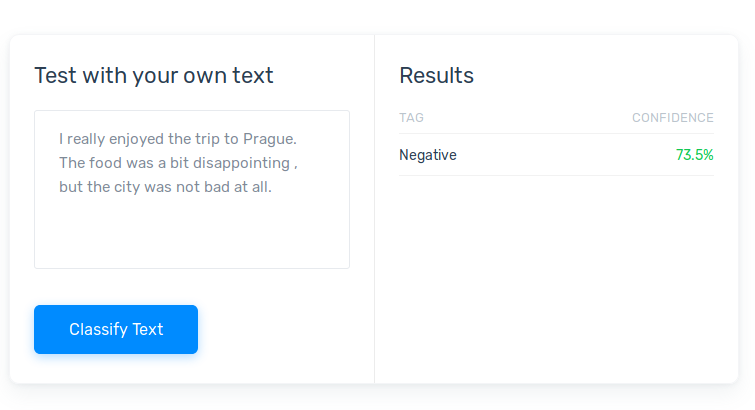
\includegraphics[width=0.7\textwidth]{figures/sentiment}
	\caption{Sentiment analysis example}
	\label{fig:sen}
\end{figure*}
Most commonly used methods:
\begin{itemize}
	\item \textbf{Rule-based}
	\item \textbf{Supervised methods} using training data, extracting features
	\item \textbf{Hybrid systems} combining the advantages of the rule based and the machine learning methods
\end{itemize}

\subsection{Question answering}
Question answering might be considered one of the oldest tasks in NLP or in AI in general with machine translation. With recent uprising products like Siri, Alexa, or Watson, it is still one of the most researched area.
If we build a question answering system, we need to take into consideration, that such system needs to handle factoid questions as well as complex request \cite{Ralph:2017}. If we want to process a factoid question such as \textit{What is the population of Europe?}, there is a clear criterion that we can define so the kind of a phrase that answers the question is clear, unlike non-factoid questions, where there may be many answers that satisfies the criterions, and sometimes it is unclear how many.

\begin{figure*}[h]
	\centering
	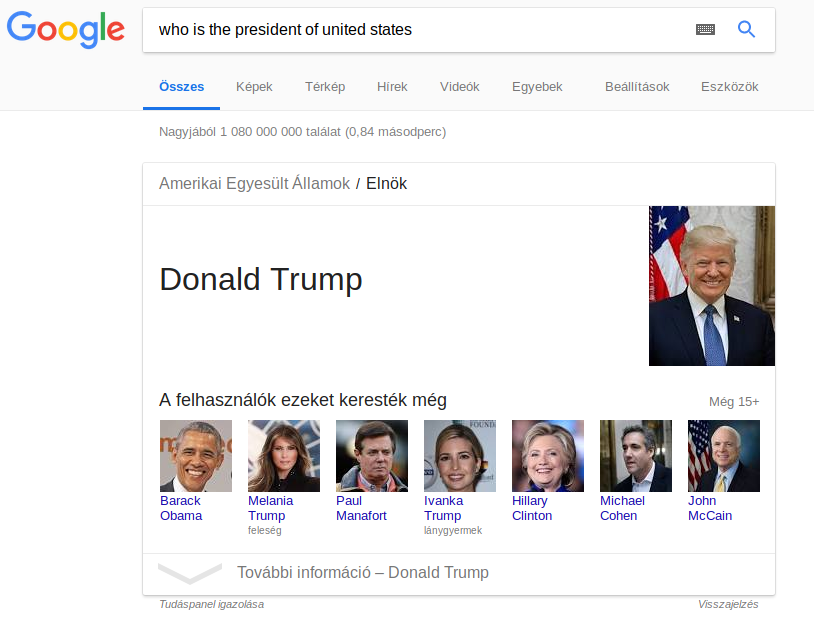
\includegraphics[width=0.7\textwidth]{figures/qagoogle}
	\caption{Question answering with google}
	\label{fig:qa}
\end{figure*}

Handling these types can be achieved using combinations of information retrieval (IR) and information extraction (IE) as described in \cite{Ralph:2017}.
IR based solutions is one of the major ones (e.g Google [\ref{fig:qa}], Watson). The main steps are:
\begin{itemize}
	\item detection the type of the questions
	\item building search queries
	\item retrieving ranked documents
	\item extracting relevant passages
	\item ranking answers
\end{itemize}

\begin{figure*}[h]
	\centering
	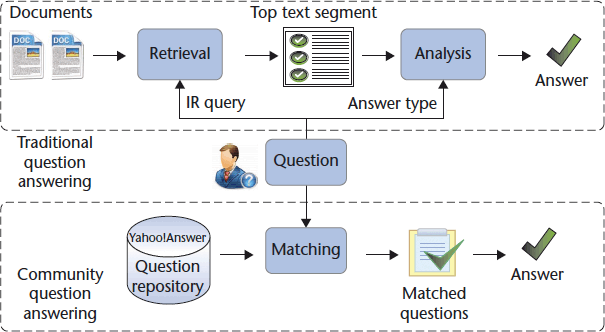
\includegraphics[width=0.7\textwidth]{figures/ie}
	\caption{Question processing system example \cite{IEsystem}}
	\label{fig:ie}
\end{figure*}

\section{Semantic parsing}
If we want to model the meaning of linguistic units, we need to map our data to some representation, so we need to choose a semantic representation. For syntactic analysis there are concepts, that are widely popular and accepted as a representation. But we cannot find such an agreement on what is the correct representation for semantic parsing.
Finding an absolute representation of semantics knowledge can be described as one of the most challenging AI task of our time, and if one could be able to construct such engine, it would be capable of \textbf{artificial general intelligence} \cite{Kornai:2018}, so we could essentially model the thinking of humans. Kornai summarized in \cite{Kornai:2018} what can be expected of a theory of semantics:
\begin{quotation}
	"our goal must be to develop a theory capable of handling the kind of commonsensical inferences that people routinely, automatically, and generally subconsciously make when answering simple questions about simple stories"
\end{quotation}

\subsection{Distributional models}
In the field of natural language processing one way of encoding semantic meaning is to use distributional models. In these models, two words are similar if they appear in the same context, and model semantic meaning as real-valued vectors. These vectors need to be constructed from a training data, and we can calculate similarity as euclidean distance between the vectors.

Lets have a look at these two sentences \textit{"The cat is walking in the bedroom"} and \textit{"A dog was running in a room"}. Words \textit{"dog"} and \textit{"cat"} have a similar semantic meaning, so if they are represented by vectors, which distance from each other is small, than we can vary the sentences \textit{"The dog is walking in the bedroom"} and \textit{"A cat was running in a room"} \cite{Bengio:2003}. The intuition is that these models want to obtain the meaning from the words around it \cite{Jurafsky:2018}. These meaning are represented by vectors, called embeddings. One of the first models build around these intuitions was introduced by Bengio \cite{Bengio:2003}. 

These word embeddings used in basically all state-of-the art systems related to natural language processing applications. Mikolov \cite{Mikolov:2013c} showed that words embeddings can be applied for vector operations, like addition or subtraction, and these operations often result in meaningful representation. Lets look at the example of vector("King") - vector("Man") + vector("Woman") \ref{fig:vecs} which results in vector("Queen"). While the usage of word embeddings brought an important breakthrough in modelling word meaning, applying them for bigger linguistics units like phrases, sentences or even whole text remained a difficult challenge even for nowadays. One of the biggest reasons for this is the additive aspect of these models: if we model A B C expression with vector v(A) + v(B) + v(C), then we represent "John killed Bill" and "Bill killed John" sentences in the same way. 

\begin{figure*}[h]
	\centering
	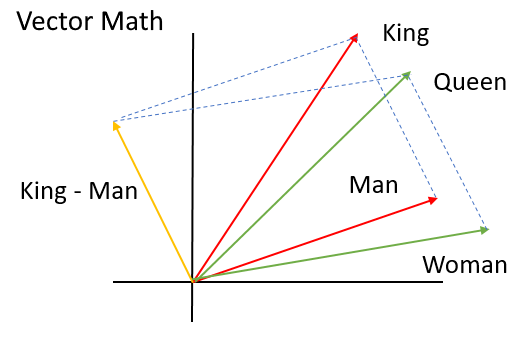
\includegraphics[width=0.7\textwidth]{figures/vecs}
	\caption{Vector addition example}
	\label{fig:vecs}
\end{figure*}

The other issue is that we know very little about the structure of a multi dimensional real-value vector (for embeddings it can be from 300 up to 1000 dimension), so it makes it very hard to understand why and when they work. So while most state-of-the art systems use word embeddings as a sole representation of meaning, and while it can be useful to encode meaning as vectors, so it can create connection from language specific and non-language specific data, we cannot deny the importance of having other semantics representations, such as graph-based ones. 

In the majority of our work, we researched graph-based solutions, where we model the meaning of lingustics unit with graphs, and the whole process can be defined with graph transformations. Next I will briefly introduce graph based formalism starting with Abstract Meaning Representations (AMR) followed by the introduction of the 4lang formalism, which will be the focus of the work, and I will go into the details in the next chapter.

\subsection{Abstract Meaning Representations}
Abstract Meaning Representation (AMR) was introduced by Banarescu\cite{Banarescu:2013} for representing the meaning of linguistic structures. They represent meaning as labeled, directed, acyclic graphs, that can be used to capture the meaning of whole sentences, so if two sentences are similar in meaning, they should be represented by similar graphs. In the past few years, we have seen multiple works related to AMR graphs, like an AMR-annotated corpus\cite{Banarescu:2013}, or multi-sentence AMR corpus \cite{OGorman2018AMRBT}, and various parsing applications \cite{DAC:2017} \cite{Vanderwende:2015}.

Nodes of AMR graphs can be represented various ways. Each node in the graph represents a semantic concept \cite{AMR:2015}, that can be either an English word, or frameset from PropBank \cite{Palmer:2005}, essentially used for abstraction. The framesets are English verbs. The AMR introduced these variables for entities, events, properties, and states. An AMR can be converted to multiple formats:
\begin{itemize}
	\item Logic format
	\item AMR format
	\item Graph format
	
	These formats can be seen on Figure \ref{fig:amr} for sentence \textit{"the boy wants to go"}, and the corresponding 4lang representation on Figure \ref{fig:4langboy}.
	
\end{itemize}

\begin{figure*}[h]
	\centering
	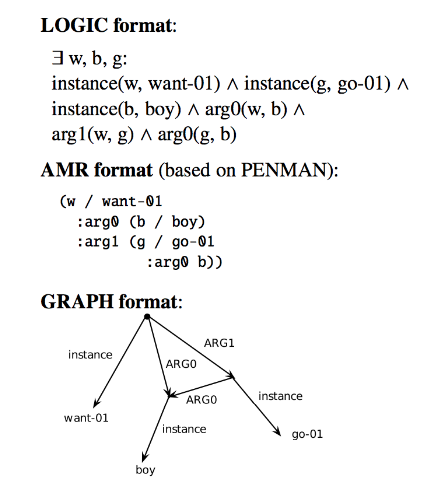
\includegraphics[height=0.4\textwidth]{figures/amr}
	\caption{Example sentence and representations}
	\label{fig:amr}
\end{figure*}

In this thesis we use the semantic parser 4lang \cite{Recski:2015b}, and unlike 4lang, AMR handles wider range of phenomenas, mostly typical of English, and AMR is not interlingua, it is heavily biased towards English \cite{Palmer:2005}, while 4lang can deal with multiple language.

\begin{figure*}[h]
	\centering
	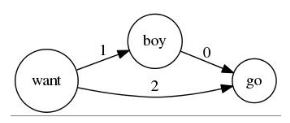
\includegraphics[width=0.3\textwidth]{figures/4langboy}
	\caption{Example sentence and representations in 4lang}
	\label{fig:4langboy}
\end{figure*}

In the next chapter, I will go into details about the 4lang formalism, and the parser itself. After I will describe our method of measuring similarities between semantic graphs, and its usage on semantic related tasks.
%----------------------------------------------------------------------------
\chapter*{4lang}\addcontentsline{toc}{chapter}{4lang}
\label{sec:4lang}
%---
The 4lang system is in the main focus of our work, in this chapter we will discuss the formalism and possible applications. 4lang also means the manually built dictionary of mapping more than 2000 words to graphs, this dictionary is described in \cite{Kornai:2013}. After discussing the main formalism of 4lang, we will demonstrate our baseline for the machine comprehension task.

\section{The formalism}
The \texttt{4lang} system of semantic representation \cite{Kornai:2015a}
represents the meaning of linguistic units (both words and phrases)
as directed graphs of syntax-independent concepts. Every node of a 4lang graph is a concept, which means that they are not taken as words, and they don't have any grammatical functions, like part-of-speech, voice, tense, etc.\cite{Recski:2016}.
Since these concepts have no grammatical attributes and no event structure, e.g.
the phrases \textit{water freezes} and \textit{frozen water} would both be
represented as \textit{water}~$\xrightarrow0$~\textit{freeze}. This also means that 4lang defines a many-to-one relation between the words and concepts. 

\textbf{4lang} formalism defines three types of edges:
\begin{itemize}
	\item \textbf{The 0-edge} represent represent attribution (\texttt{dog
		$\xrightarrow0$ large}), hypernymy (\texttt{dog $\xrightarrow0$ mammal}) and unary predication (\texttt{dog  $\xrightarrow0$ bark})
	\item \textbf{1- and 2-edges} those representing binary relations are connected to their arguments
	via edges labeled \texttt{1} and \texttt{2}, e.g \texttt{cat $\xleftarrow1$ catch $\xrightarrow2$ mouse}. Binaries that are shown with uppercase are binaries that must have two outgoing edges as shown in Figure \ref{fig:4langbin}. If we look at the sentence \textit{"Kinga broke Adam's bike"}, and the corresponding graph shown in Figure \ref{fig:4langbin}, if the 0-connection wouldn't be present between \textit{Kinga} $\xrightarrow0$ break, that would mean we consider that the relationship depend on whether the object of breaking is established or not. So in \textbf{4lang} the connection of 0-edge is present between a subject and a predicate regardless of the other arguments.
\end{itemize}

\begin{figure*}[h]
	\centering
	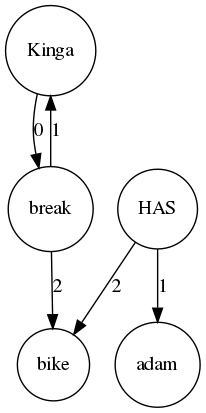
\includegraphics[height=0.5\textwidth]{figures/binary4lang}
	\caption{4lang with binaries}
	\label{fig:4langbin}
\end{figure*}

The example in
Figure~\ref{fig:bird} shows the \texttt{4lang} definition of the
concept \texttt{bird}. This definition was built manually, as part of
the \texttt{4lang} dictionary \cite{Kornai:2013}, but similar
definitions have been created automatically from definitions of
monolingual dictionaries such as Longman, using the
\texttt{dict\_to\_4lang} tool \cite{Recski:2016d}.

The open-source 4lang pipeline\footnote{\url{https://github.com/kornai/4lang}}
contains tools for generating
directed graphs from raw text by mapping dependency edges in the output of the
Stanford parser \cite{deMarneffe:2006} to \texttt{4lang} subgraphs over
concepts corresponding to each word of the original sentence. The Standford parser builds a dependency tree from the raw text that captures the syntactical relations between the linguistics units. 4lang graph construction involves mapping from these relations to 4lang semantics graphs, assigning the dependencies to 4lang subgraphs. The mapping is presented in Table \ref{table:mapping}, and an example is shown for sentence \textit{"I like swimming"} in Figure \ref{fig:swimmingdep}, where we can see the dependency tree coming out of the Standford parser, and the corresponding 4lang graph is present in Figure \ref{fig:swimming}, where the mapping from the dependency tree to \textbf{4lang} graph is done. 

\begin{table}
	\centering
	%\small
	\begin{tabular}{lc}
		\toprule
		Dependency & Edge \\
		\midrule
		amod & \multirow{7}{*}{\edge{$w_1$}{0}{$w_2$}} \\
		advmod & \\
		npadvmod & \\
		acomp & \\
		dep & \\
		num & \\
		prt & \\
		\midrule
		nsubj & \multirow{4}{*}{\twoedges{$w_1$}{1}{0}{$w_2$}} \\
		csubj & \\
		xsubj & \\
		agent & \\
		\midrule
		dobj & \multirow{6}{*}{\edge{$w_1$}{2}{$w_2$}} \\
		pobj & \\
		nsubjpass & \\
		csubjpass & \\
		pcomp & \\ 
		xcomp & \\
		\midrule
		appos & \twoedges{$w_1$}{0}{0}{$w_2$} \\
		\midrule
		poss & \multirow{2}{*}{$w_2\xleftarrow1$ \texttt{HAS} $\xrightarrow2w_1$} \\
		prep\_of & \\
		\midrule
		tmod & $w_1\xleftarrow1$ \texttt{AT} $\xrightarrow2w_2$ \\
		\midrule
		prep\_with & $w_1\xleftarrow1$ \texttt{INSTRUMENT} $\xrightarrow2w_2$ \\
		\midrule
		prep\_without & $w_1\xleftarrow1$ \texttt{LACK} $\xrightarrow2w_2$ \\
		\midrule
		prep\_P & $w_1\xleftarrow1$ \texttt{P} $\xrightarrow2w_2$ \\
		\bottomrule
	\end{tabular}
	\caption{Mapping from Stanford dependency relations to 4lang subgraphs \cite[p. 12.]{Recski:2018}.}
	\label{table:mapping}
\end{table}

\begin{figure*}[h]
	\centering
	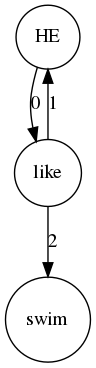
\includegraphics[height=0.5\textwidth]{figures/swimming}
	\caption{4lang example of a sentence}
	\label{fig:swimming}
\end{figure*}

\begin{figure*}[h]
	\centering
	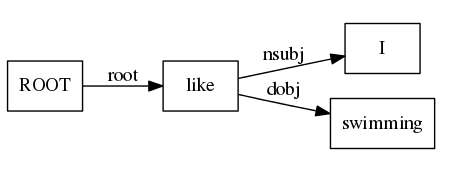
\includegraphics[width=0.5\textwidth]{figures/swimmingdep}
	\caption{Standford example of a sentence}
	\label{fig:swimmingdep}
\end{figure*}


\subsection{Expansion}
Optionally, the \texttt{4lang} system allows us to \textit{expand}
graphs, a process which unifies the graph with the definition graphs of
each concept. The implementation is written in the \textbf{dict\_to\_4lang} module, that extends the functionality of the discussed \textbf{text\_to\_4lang} pipeline with dictionaries. 4lang takes advantage of this, and implements the expansion step, which essentially is joining the definitions graphs to the main graph. This allow us to build a larger graph, that contains more information, and allow us to model the text better by simply adding the definition of words.

Let us look at the example sentence \textit{"My poor wife"}, that results the graph shown in Figure \ref{fig:mypoor}. If we are ready to make an assumption that taking word definitions into account results us a better model, and with this method we can have higher similarites between graphs whose sentences are also similar, than looking at the word poor definition is: \textit{having very little money and not many possessions}, we can build a definition graph and essentially join the two graphs together doing this for every word in the sentence resulting in a merged graph Figure \ref{fig:mypoorexpanded}. If we look at the graph, it is clear that the expanded graph gives us much more accurat context and definition. Our work was build around the expanded graph, and we will se that how better it actually performs on a real task. This will be the main topic of the next chapter.

\begin{figure}
	\centering
	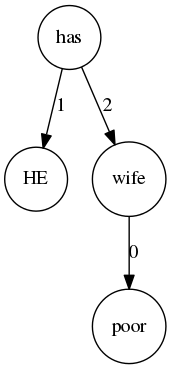
\includegraphics[scale=0.5]{figures/mypoor}
	\caption{4lang definition of sentence \textit{"My poor wife"}.}
	\label{fig:mypoor}
\end{figure}

\begin{figure}
	\centering
	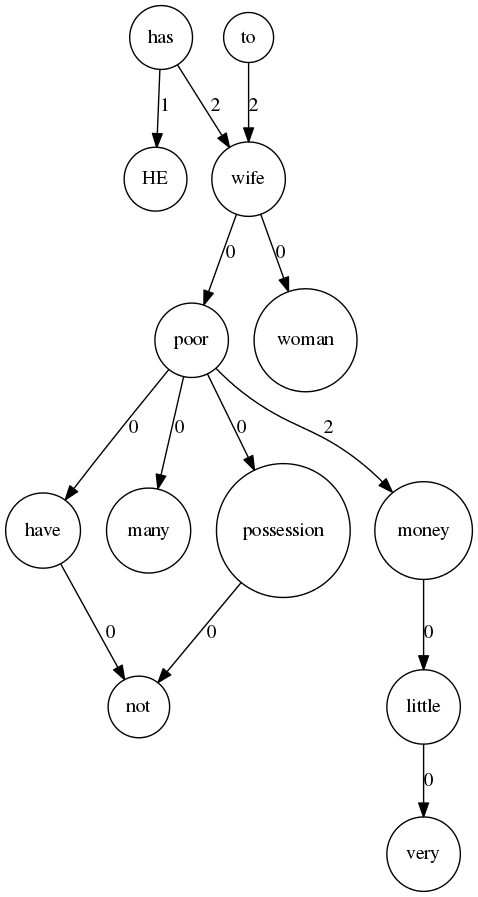
\includegraphics[scale=0.5]{figures/mypoorexpanded}
	\caption{4lang definition of expanded sentence \textit{"My poor wife"}.}
	\label{fig:mypoorexpanded}
\end{figure}

The beginning of our research we put a high emphasis on generating graphs from text with a highly automated method, so besides being an open-source software library,
the \texttt{4lang} we made the accessible via a public
REST API at \url{http://hlt.bme.hu/4lang}. We can generate graphs with raw text by calling the service. Currently our service have multiple endpoints, with each of them representing different methods.
If you interested in only processing a single sentence, you can call the following endpoints:

\begin{itemize}
	\item \textbf{/sendef} - Returns the graphs built from the sentence.
\item \textbf{/senexp} - Returns the graphs, where the word's definition has been added to the graph.
\item \textbf{/senabs} - Calling this function, we defined some rules, where we can build a more abstract graph using the definitions, this is more of a future work, I will talk about it  a bit in the last chapter.
\end{itemize}
You can get a word's definition by calling the defined endpoint:
\begin{itemize}
	\item \textbf{/definition} - Returns the graphs built from the word's definition.
\end{itemize}


\begin{figure}
	\centering
	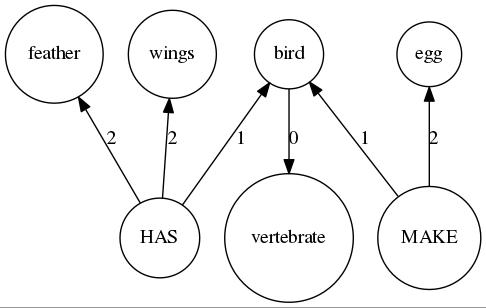
\includegraphics[scale=0.5]{figures/bird}
	\caption{4lang definition of \texttt{bird}.}
	\label{fig:bird}
\end{figure}

Graphs generated by the \texttt{4lang} parser have previously been used
successfully in measuring semantic similarity. The current state of the
art system on the \texttt{SimLex-999} benchmark \cite{Hill:2014a}
outperforms previous top systems by utilizing a simple similarity metric
between \texttt{4lang} definitions of pairs of English words
\cite{Recski:2016c}, this was the main idea of trying it in a different task with a different state-of-the-art system.

In the next chapter, I will briefly discuss the machine comprehension challenge, and I will introduce our baseline method for solving it. After that We will present how it is applicable to an already working system.
\chapter{Yuanfudao system}
\label{chap:yuanfudao}
On the 2018 Semeval Task \textit{Machine comprehension using commonsense knowledge} competition the \texttt{Yuanfudao} \cite{Wang:2018} system reached second place with $83.95\%$ accuracy on the test data.

% Yuanfudao introduction
\section{The original system}

The \texttt{Yuanfudao} system implements a Three-way Attentive Network (TriAN), an ensemble of three LSTMs augmented with various attention mechanisms, to model for each question interactions between question, possible answers, and the passage that may or may not contain the correct answer to the question.

The system was implemented using python programming language and the \texttt{pytorch} package for the implementation of the neural network. The source code is available on Github\footnote{\url{https://github.com/intfloat/commonsense-rc}}.

% Yuanfudao preprocess

\subsection{Preprocessing}
This system processes the input data as follows:

\begin{enumerate}
	\item Using the \texttt{spacy} package's tokenizer function it generates the part of speech (pos) tag, named entity recognition (ner) tag and the lemma for each word in the passage, and the pos tags of the questions.
	\item It assigns a number representation and an offset for each word in the passage, questions and answers.
	\item It also saves the ids of the passages, questions and answers and whether the answer was correct.
	\item The preprocessor finds the words and lemmas in the questions and answers, that also occurred in the passage's word and lemma list. 
	\item It stores each word's frequency using the \texttt{wikiwords} library.
	\item It  establishes the \textit{ConceptNet} relation between the words of the passage and question and also between the words of the passage and answer.
	\item The preprocessor saves all this data to their respective json files.
\end{enumerate}


\paragraph*{Conceptnet} \cite{Speer:2017} \\

\textit{ConceptNet} plays a major part of the \texttt{Yuanfudao} system, as it was shown in the original paper \cite{Wang:2018}. This is a metric  used to show the possible relationship between two words. These relations could be "RelatedTo", "IsA", "Synonym", "PartOf" etc. 

The \textit{ConceptNet} itself is a large graph of general knowledge that has shown to be affective at determining word relations.

The preprocessor compares the words in the passage with the words in the "query" (question or answer) using \textit{ConceptNet} and stores only one of the matches per word, if there were any.

% System description

\subsection{System description}

An overview of the original system is reproduced in Figure~\ref{fig:dnn}.
\begin{figure}[h!]
	\centering
	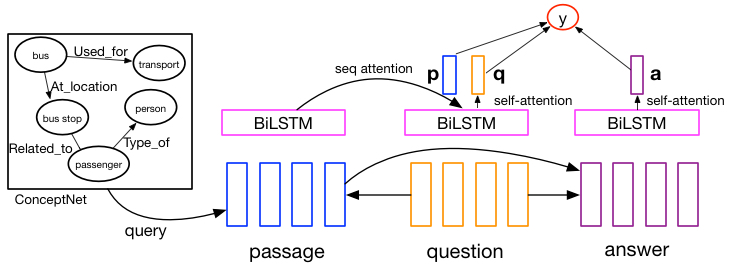
\includegraphics[scale=0.5]{TriAN.jpg}
	\caption{Structure of the original network \cite{Wang:2018}}
	\label{fig:dnn}
\end{figure}

This system is a deep learning neural network consisting of embeddings, recurrent neural networks and attention mechanisms.

First the inputs generated in the preprocessing phase go through three embedding layers, each corresponding to the passage, question and answer respectively. There are also pos-embedding, ner-embedding and rel-embedding layers. The pos-embedding gets the passage's and the question's pos tags as its input, the ner-embedding layer gets the passage's ner-tags and the relation-embedding gets the relationship vectors generated using the \textit{ConceptNet}. This input embedding layer is shown in Figure~\ref{fig:embedding}.
\begin{figure}[h!]
	\centering
	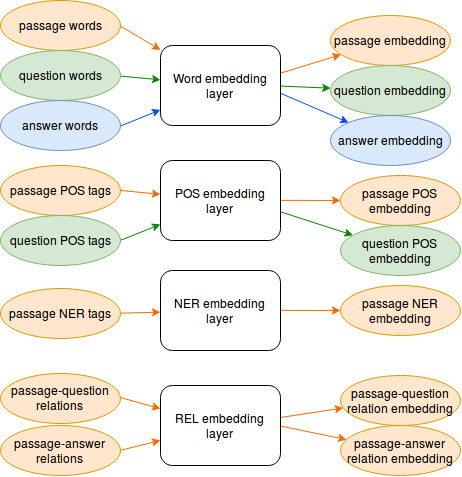
\includegraphics[scale=0.5]{TriAN_embeddings.jpg}
	\caption{Structure of the input embedding layers.}
	\label{fig:embedding}
\end{figure}

The word embeddings' outputs are paired up (passage-question, answer-question, answer-passage) and go through a so called \textit{sequence attention matching layer}.
The sequence attention matching layer at its core uses the bmm function in \texttt{pytorch} which performs a batch matrix-matrix product of the input matrices.
This way it "matches" the two inputs together. This is shown in Figure~\ref{fig:attention_match}.
\begin{figure}[h!]
	\centering
	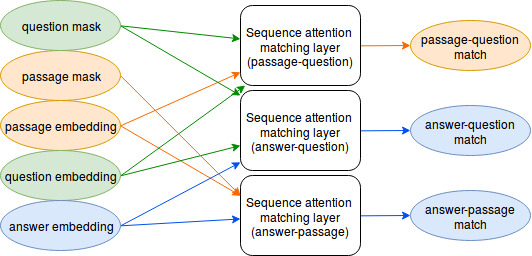
\includegraphics[scale=0.5]{TriAN_attention_match.jpg}
	\caption{Structure of the \textit{sequence attention matching layers}.}
	\label{fig:attention_match}
\end{figure}

The system uses dropouts after the embedding and sequence attention matching layer layers to avoid over-fitting.

These layers are followed by three \textit{stacked bidirectional RNN layer}, each corresponding to the passage, question and answer respectively. It differs from the standard bidirectional RNN layer in one aspect: it can concatenate the hidden states of the RNN. By default the type of the RNN is LSTM, but it can also be GRU. Their inputs are sort of self explanatory. The passage's stacked bidirectional RNN layer gets the passage's word embedding layer, the output of the sequence attention matching layer for the passage-question input pair, the passage's pos- and ner-embedding layers, the word frequency tensor created with the \texttt{wikiword} library, and the two relation-embedding layer's output. The question's stacked bidirectional RNN layer expects the question's word and pos-embedding outputs on its input. The answer's stacked bidirectional RNN layer's inputs are the answer's word embedding output and  the output of the sequence attention matching layer for the answer-question and the answer-question input pairs. These RNN layers are shown in the Figure~\ref{fig:rnn}.
\begin{figure}[h!]
	\centering
	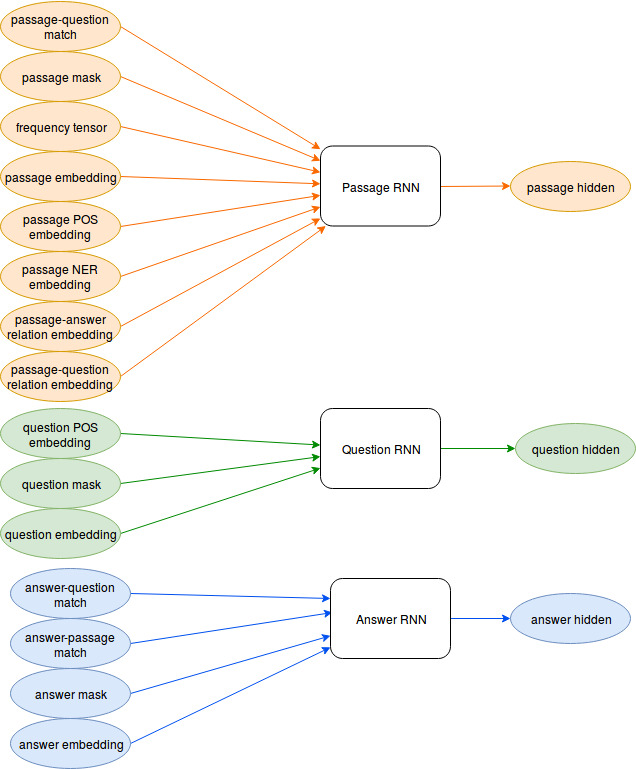
\includegraphics[scale=0.4]{TriAN_rnn.jpg}
	\caption{Structure of the \textit{stacked bidirectional RNN layers}.}
	\label{fig:rnn}
\end{figure}
This layer implicitly uses a dropout rate for regularization.

The question's and the answer's stacked bidirectional RNN layer's outputs are used in two \textit{linear sequence attention layers}, or better known as \textit{self-attention layers over a sequence} for the question and the answer respectively. This layer is basically a linear layer slightly modified, so the infinite outputs are masked and it uses a softmax function at its output.

The passage's stacked bidirectional RNN layer's output is used differently. The system passes it and the question's \textit{stacked bidirectional RNN layer's} output to a \textit{bilinear sequence attention layer}, which is similarly to the sequence attention matching layer uses the bmm function as its core function.

The two linear sequence attention layer's and the bilinear sequence attention layer's output is passed through a weighted averaging function with their respective stacked bidirectional RNN layer's output. This part of the network is shown in Figure~\ref{fig:sequence_attention}.
\begin{figure}[h!]
	\centering
	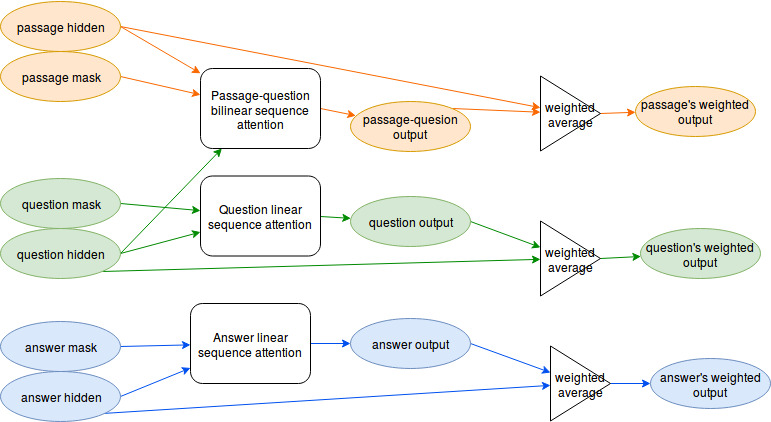
\includegraphics[scale=0.5]{TriAN_sequence_attention.jpg}
	\caption{Structure of the sequence attention layer\\and the following weighted average function.}
	\label{fig:sequence_attention}
\end{figure}

The averaged passage output is passed though a \textit{linear feed forward layer} than multiplied by the answer's averaged output. The question's averaged output is passed though an other linear feed forward layer than multiplied by the answer's averaged output. At the end its all summed and sigmoid function used at its output. The output in this case is whether the answer was correct to the given question or not. This last section is at Figure~\ref{fig:output}.
\begin{figure}[!htb]
	\centering
	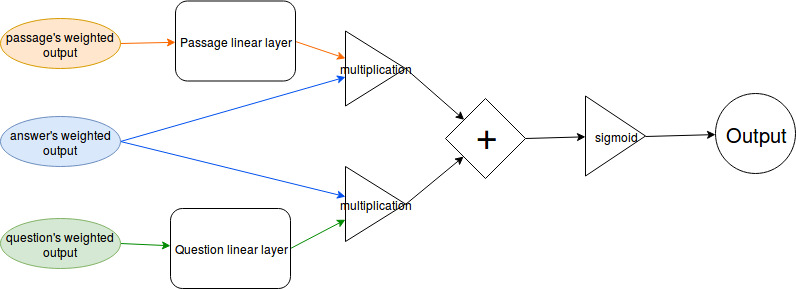
\includegraphics[scale=0.5]{TriAN_output.jpg}
	\caption{Structure of the output of the network.}
	\label{fig:output}
\end{figure}


\subsection{Parameters}
\begin{minipage}{\textwidth}
The \texttt{Yuanfudao} system has these following command line arguments:
\begin{itemize}
	\item \textbf{GPU}: the training of the system can be done on GPU which is much faster than training it on CPU
	\item \textbf{using cuda}: \texttt{pytorch} can support CUDA for parallelization. The system uses CUDA by default.
	\item \textbf{optimizer}: the optimizer function can be adamax (default) or SGD
	\item \textbf{RNN type}: the RNN used by the system can be LSTM or GRU
	\item \textbf{dropout rate}: there are separate dropout rates for embeddings and RNNs
	\item \textbf{embedding dimension}: each embedding dimension in the system can be manually set
	\item \textbf{gradient clipping}: the gradient clipping threshold can be set
	\item \textbf{epoch}
	\item \textbf{learning rate}
	\item \textbf{batch size}
	\item \textbf{random seed}
	\item other parameters related to input handling, RNN settings and testing
\end{itemize}
You can read about the deep learning related arguments and their functions in Chapter \ref{chap:deep}.
\end{minipage}

\subsection{Learning curve}
\begin{minipage}{\linewidth}
Without the recommended pretraining (Figure~\ref{fig:learning_curve}):
\begin{itemize}
	\item Max dev accuracy: $82.7\%$ reached in the 26th epoch
	\item Train accuracy: $97.7\%$ reached in the 26th epoch
	\item Max train accuracy: $99.8\%$ reached in the 50th epoch
	\item Last dev accuracy: $81.9\%$
	\item Average dev accuracy after ten epochs: $81.9\%$
\end{itemize}
\end{minipage}
\begin{figure}[!htb]
	\centering
	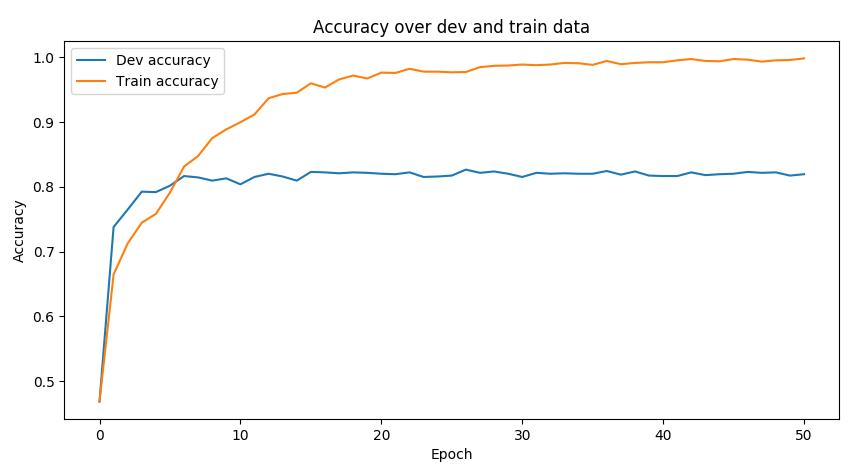
\includegraphics[scale=0.5]{learning_curve.jpg}
	\caption{Learning curve without pretraining.}
	\label{fig:learning_curve}
\end{figure}

\begin{minipage}{\linewidth}
With the recommended pretraining(Figure~\ref{fig:learning_curve2}):
\begin{itemize}
	\item Max dev accuracy: $82.5\%$ reached in the 38th epoch
	\item Train accuracy: $99\%$ reached in the 38th epoch
	\item Max train accuracy: $99.7\%$ reached in the 50th epoch
	\item Last dev accuracy: $82.2\%$
	\item Average dev accuracy after ten epochs: $81.9\%$
\end{itemize}
\end{minipage}
\begin{figure}[!htb]
	\centering
	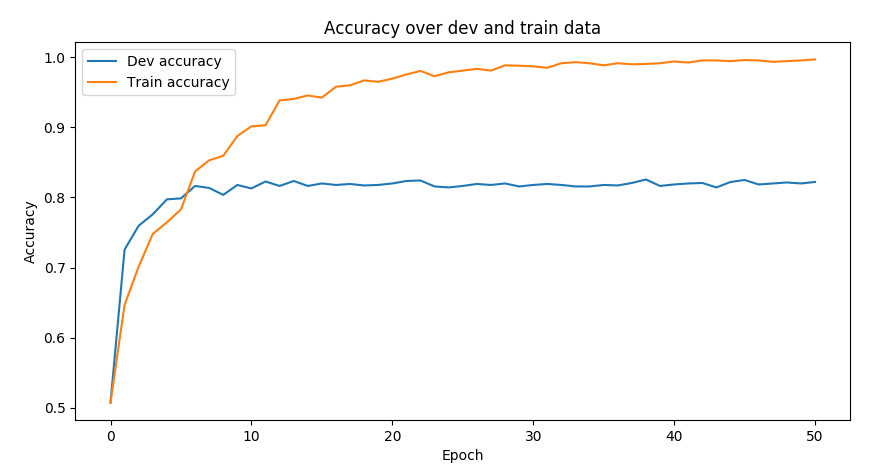
\includegraphics[scale=0.5]{learning_curve2.jpg}
	\caption{Learning curve with pretraining.}
	\label{fig:learning_curve2}
\end{figure}

As you can see there is no significant difference between the learning curve with or without pretraining.

\section{Modifications}
Our modifications are available on Github\footnote{\url{https://github.com/GKingA/commonsense-rc}}.

We modified the preprocessing part of the system to incorporate the similarity calculating method from Chapter ~\ref{chap:comprehension}. The most straightforward way of incorporating our metric into the system is by creating vectors similar to those representing \textit{ConceptNet} relations between words of a passage and words in each answer candidate. Since these vectors represent
word-to-word relationships, we measure the support between pairs of \texttt{4lang} definition graphs, and for each word in the passage we take the maximum support score over all words of the answer candidate. Elements of a vector for a passage $P$ and a possible answer $A$ are hence defined as:

\[S^{(P, A)}_i = \max_{A_j \in A} S(P_i, A_j)\]

Elements of a vector for a passage $P$ and a question $Q$ are defined as:

\[S^{(P, Q)}_i = \max_{Q_j \in Q} S(P_i, Q_j)\]

Elements of a vector for a question $Q$ and an answer $A$ are defined as:

\[S^{(Q, A)}_i = \max_{A_j \in A} S(Q_i, A_j)\]

We used these new input vectors as the input of a new \texttt{4lang} embedding layer that functions similarly to the other embedding layers. It is shown at Figure~\ref{fig:4lang_embedding}. The input of this layer is 101 dimensional, since the similarities are on a scale to 0 to 100.

\begin{figure}[h!]
	\centering
	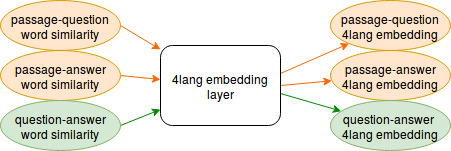
\includegraphics[scale=0.5]{4lang_embedding.jpg}
	\caption{\texttt{4lang} embedding layer.}
	\label{fig:4lang_embedding}
\end{figure}

The outputs of this layer is passed to the RNN layers. This is depicted at Figure~\ref{fig:rnn_4lang}.

\begin{figure}[h!]
	\centering
	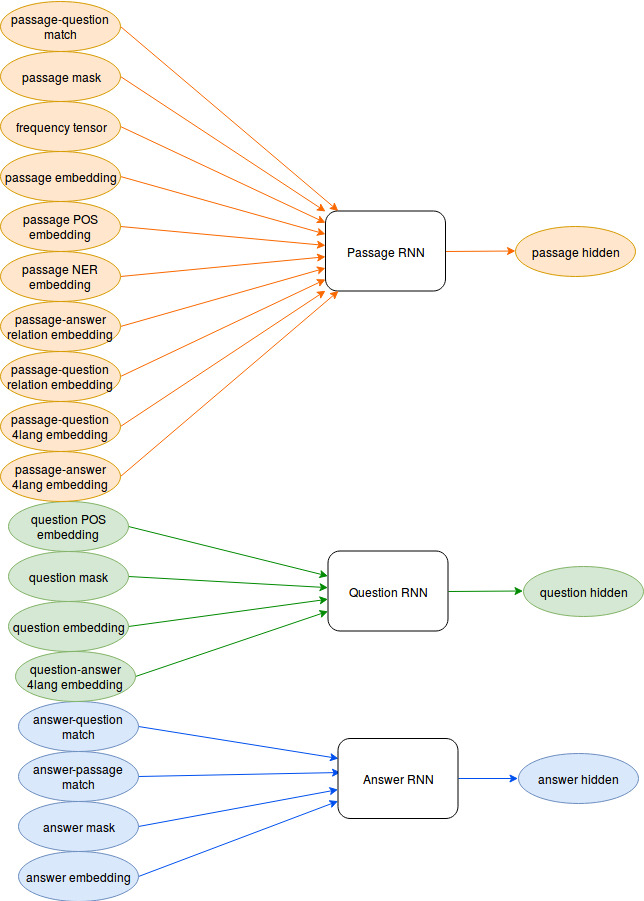
\includegraphics[scale=0.4]{TriAN_rnn_with_4lang.jpg}
	\caption{Structure of the modified \textit{stacked bidirectional RNN layers}.}
	\label{fig:rnn_4lang}
\end{figure}

Since we also wanted to see how the system changes if we replace \textit{ConceptNet} relations with our metric, we also trained systems without \textit{ConceptNet} rel-embeddings.

\FloatBarrier

\section{The results}
The original \texttt{Yuanfudao} \cite{Wang:2018} publication said its system was able to reach $83.95\%$ accuracy on the test data. We were only able to reproduce a $80.3\%$ accuracy on the test set and $82.5\%$ on the development set with the recommended pretraining on the \texttt{RACE} \cite{Lai:2017} dataset. We will take these results as our bases of the comparison.

We tested our model by turning on and off the usage of \textit{ConceptNet} and \texttt{4lang}. There were 4 combinations: using neither, just \textit{ConceptNet}, just \texttt{4lang} and both.

\begin{table}[h!]
	\centering
	\begin{tabular}{ | l | c | r | }
		\hline
		model & dev & test \\ \hline \hline
		pretrained TriAN, no ConceptNet & 83.7\% & 81.9\% \\ \hline
		pretrained TriAN, with ConceptNet & 82.5\% & 80.3\% \\ \hline
		pretrained TriAN, with 4lang & 84.2\% & 81.5\% \\ \hline
		\textbf{pretrained TriAN, with both} & \textbf{83.4\%} & \textbf{82.9\%} \\ \hline
		TriAN, no ConceptNet & 82.8\% & 80.2\% \\ \hline
		TriAN, with ConceptNet & 82.7\% & 80.5\% \\ \hline
		TriAN, with 4lang & 83.2\% & 80.9\% \\ \hline
		TriAN, with both & 83.1\% & 80.8\% \\ \hline
	\end{tabular}
	\caption{Effect of \texttt{4lang} and \texttt{ConceptNet} on results}
	\label{tabl:res}
\end{table}

It is evident that without pretraining the Yuanfudao system performs best if we use the relation scores calculated from \texttt{4lang} graphs instead of the \textit{ConceptNet} relationships.
After pretraining the network on the \texttt{RACE} dataset the results show that using both of the relation metric is most beneficial.

%\listoffigures\addcontentsline{toc}{chapter}{?br?k jegyz?ke}
%\listoftables\addcontentsline{toc}{chapter}{T?bl?zatok jegyz?ke}


\bibliography{mybib}
\addcontentsline{toc}{chapter}{Irodalomjegyzék}
\bibliographystyle{plain}

\label{page:last}
\end{document}

